\section{Preliminaries}\label{sec2}
\subsection{Model of robots}
Consider a swarm $\mathcal{N}$ that contains $n$ robots labelled $i\in\left\{1,...,n\right\}$. We model the swarm as a directed sensing graph $\mathcal{G}=\left(\mathcal{V},\mathcal{E}\right)$, where vertex set $\mathcal{V} = \left\{1,..., n\right\}$ represents the robots, and edge set $\mathcal{E}\subseteq\mathcal{V}\times \mathcal{V}$ contains the pairs of robots $\left(i, j\right)\in\mathcal{E}$ for which robot $i$ can sense robot $j$. We denote $\mathcal{N}_i=\left\{j\in\mathcal{V}|\left(i,j\right)\in\mathcal{E}\right\}\subset\mathcal{V}$ as the set of $n_i$ neighbours of a robot $i$ in $\mathcal{G}$.

\begin{figure}
    \centering
    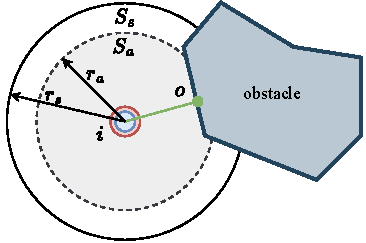
\includegraphics[width=0.45\textwidth]{paper2/images/model.pdf}
    \caption{Illustration of a robot with a local range sensor. Each robot is equipped with a local sensor with sensing area $S_s$ (solid while circle) being a circular disk within radius $r_s$. Additionally, alert area $S_a$ (dashed gray circle) is a circular disk within radius $r_a$, with $r_a\leq r_s$, which is the zone that robot will active the repulsive force to avoid collision. The set~$\mathcal{M}_i=\{o\}$ (green) is the nearest point from robot $i$ to obstacle.}
    \label{fig:1model}
\end{figure}

\begin{figure*}
    \centering
    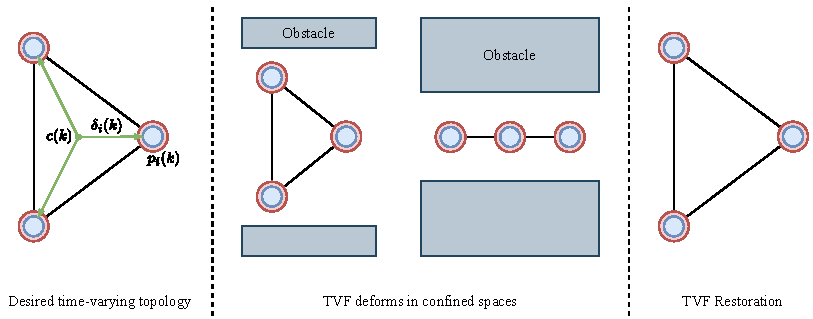
\includegraphics[width=0.9\textwidth]{paper2/images/problem.pdf}
    \caption{Schematic diagram of time-varying formation in the confined space}
    \label{fig:1problem}
\end{figure*}
In this study, the robots' dynamics are expressed in discrete time. The position, velocity, and control input of robot $i$ at time $t(k) = k\tau$ are denoted as $p_i(k), v_i(k), u_i(k) \in \mathbb{R}^3$, respectively, where $\tau$ represents the time step. The robots in the swarm are identical, each with a body radius $r$. Each robot $i$ is equipped with an inertial measurement unit (IMU) to determine its position and orientation in a desired direction, a range sensor, and a wireless ad-hoc network module for peer-to-peer communication with other robots. In this study, the communication delay between any two robots is assumed to be negligible~\cite{AlonsoMora2018,9527169}. Additionally, each robot is equipped with a circular sensor~\cite{8716301} that offers a $360^\circ$ field of view of the environment and can observed a maximum area $S_s$ within a radius $r_s$, as depicted in Fig.~\ref{fig:1model}. The set $\mathcal{M}_i(k) = \left\{o\right\}$ represents the observed obstacle points $o$ which is the nearest point on the obstacle's boundary at time $t(k)$. Additionally, a circular with the radius $r_a$ is denoted as an alert area that actives repulsive forces when robot $i$ sensing obstacles or its neighbors.

According to~\cite{Dong2015}, assuming that every robot in the swarm obeys a discrete linear system, given by
\begin{equation}
    x_i(k+1)=A_ix_i(k) + B_iu_i(k)
    \label{eqn:1model}
\end{equation}
where $A_i$ and $B_i$ are constant matrices. We consider the system to represent a robot with an underlying acceleration controller. The input $u_i$ is an acceleration command, and the state $x_i=\left[p_i,v_i\right]^T\in\mathbb{R}^6$ is a vector containing the position and velocity. The velocities and accelerations of the robots are bounded by constant vectors, i.e. $\left\Vert v_i(k)\right\Vert\leq v_\text{max}$ and $\left\Vert u_i(k)\right\Vert\leq u_\text{max}$.

\subsection{Problem formulation}

This paper addresses the safe formation control of time-varying formation (TVF) in confined space. The primary challenges addressed are:
\begin{enumerate}
    \item Ensuring collision-free navigation for the TVF, even when in the limited space environment.
        \item Incorporating an event-triggering mechanism into the TVF control, allowing the formation to deform to another safe configuration.
\end{enumerate}

Fig.~\ref{fig:1problem} provides the general schematic diagram of the research problem tackled in this study. Initially, the desired configuration assigned to the TVF is denoted $\delta_0$. At time $k$, the TVF can maintain the initial topology, i.e. $\delta(k)=\delta_0$. However, the confined space does not allow the formation maintaining topology $\delta_0$ due to the potential collision. As a result, a new topology is triggered to be applied depending on the surrounding space. Once the confined space is not detected by the robot, the initial topology $\delta_0$ of the formation is restored. With the proposed control approach, the formation configuration can be effectively managed. During the movement of the TVF, collaborative and collision avoidance controls are driven by the APF term in the proposed control strategy.

\begin{definition}\label{def_tvf}
(Time-Varying Formation~\cite{Dong2015,Dong2016} - TVF).  Let $\delta(k)=\left[\delta_1(k),...,\delta_n(k)\right]^T$ be a bounded time-varying vector that describes the desired formation configuration. The formation is said to achieve a TVF $\delta(k)$ if all robot $i$ in the formation satisfy:
\begin{equation}
    \lim_{k\to\infty}\sum_{i=1}^n\left\Vert p_i(k)-\delta_i(k)-c(k)\right\Vert=0,\quad\forall i\in\left\{1,...,n\right\}
\end{equation}
where $c(k)$ is called a formation center in the time $k$.
\end{definition}

\begin{definition}\label{def_pro}
(Safe Formation Control). Given the TVF as defined in Definition~\ref{def_tvf}, the safe formation control of TVF is said to be realized for any robot $i$ in the formation if the following conditions are simultaneously satisfied:
\begin{enumerate}
    \item Formation configuration
\begin{equation}
    \lim_{k\to\infty}\sum_{i=0}^n{\left\Vert\left(p_i(k)-\delta_i\right) - \left(p_j(k)-\delta_{j}\right)\right\Vert}=0
    \label{eqn:1form}
\end{equation}
for all $i,j\in\left\{1,...,n\right\}$, $i\neq j$.
%     \item Task completion
% \begin{equation}
%     \lim_{k\to T}\left\Vert\dfrac{1}{n}\sum_{i=1}^np_i-p_g\right\Vert=0
%     \label{eqn:1goal}
% \end{equation}
% where $T$ is a finite time, $p_g$ is the target position.
    \item Safe distance between robots
\begin{equation}
    \left\Vert p_i(k)-p_j(k)\right\Vert > 2r
    \label{eqn:1col}
\end{equation}
for all $i\in\left\{1,...,n\right\}$.
    \item Safe distance from obstacles
\begin{equation}
    \left\Vert p_i(k)-m\right\Vert > r
    \label{eqn:1obs}
\end{equation}
for all $i\in\left\{1,...,n\right\}$, and for all $m\in\mathcal{M}_i(k)$. 
\end{enumerate}
\end{definition}

\begin{remark}
According to the discrete linear model presented in~\eqref{eqn:1model}, this study primarily focuses on the changes in the position and velocity status of the robot. Based on Definition~\ref{def_tvf}, when~\eqref{eqn:1form} is established, robots reach the desired position, achieving the desired configuration. 
% Simultaneously, the velocity tends to zero once the tasks are completed~\eqref{eqn:1goal}. 
The establishment of \eqref{eqn:1col}~--~\eqref{eqn:1obs} ensure that the robot will not collide with obstacles or other robots in the formation, respectively.
\end{remark}

\subsection{Formation configurations}\label{sec:config}
Formation configurations are emerging while robots are cooperating and interacting with the confined space environments. In this study, we categorize formation configurations into two primary configurations:
\begin{enumerate}
    \item \textit{Original configuration:} This formation configuration is maintained if any surrounding space is large enough to maintain the originally defined configuration or to transform it by contraction. The configuration can be a V-shape, a polygon, or others.
        \item \textit{Straight line configuration:} This formation configuration is performed when the robot does not have enough space to maintain the original configuration, forcing it convert to this form for safety assurance~\cite{Fu2020}. This configuration is constructed by having a robot follow and keep desired distance from its leader.
\end{enumerate}